\documentclass[11pt]{report} % Tipo de documento

% Paquetes y configuraciones adicionales
\usepackage{graphicx}
\usepackage[export]{adjustbox}
\usepackage{caption}
\usepackage{float}
\usepackage{titlesec}
\usepackage{geometry}
\usepackage[hidelinks]{hyperref}
\usepackage{titling}
\usepackage{titlesec}
\usepackage{parskip}
\usepackage{wasysym}
\usepackage{tikzsymbols}
\usepackage[spanish]{babel}

% Configuración de los títulos de las secciones
\newcommand{\subtitle}[1]{
  \posttitle{
    \par\end{center}
    \begin{center}\large#1\end{center}
    \vskip0.5em}
}

% Configura los márgenes
\geometry{
    left=2cm,   % Ajusta este valor al margen izquierdo deseado
    right=2cm,  % Ajusta este valor al margen derecho deseado
    top=3cm,
    bottom=3cm,
}

% Configuración de los títulos de las secciones
\titlespacing{\section}{0pt}{\parskip}{\parskip}
\titlespacing{\subsection}{0pt}{\parskip}{\parskip}
\titlespacing{\subsubsection}{0pt}{\parskip}{\parskip}

% Redefinir el formato de los capítulos y añadir un punto después del número
\makeatletter
\renewcommand{\@makechapterhead}[1]{%
  \vspace*{0\p@} % Ajusta este valor para el espaciado deseado antes del título del capítulo
  {\parindent \z@ \raggedright \normalfont
    \ifnum \c@secnumdepth >\m@ne
        \huge\bfseries \thechapter.\ % Añade un punto después del número
    \fi
    \interlinepenalty\@M
    #1\par\nobreak
    \vspace{10pt} % Ajusta este valor para el espacio deseado después del título del capítulo
  }}
\makeatother

% Configura para que cada \chapter no comience en una pagina nueva
\makeatletter
\renewcommand\chapter{\@startsection{chapter}{0}{\z@}%
    {-3.5ex \@plus -1ex \@minus -.2ex}%
    {2.3ex \@plus.2ex}%
    {\normalfont\Large\bfseries}}
\makeatother

\begin{document}

% Portada del informe
\title{Practicaa 08. Configurando un Firewall con DMZ}
\subtitle{Seguridad de Sistemas Informáticos}
\author{Cheuk Kelly Ng Pante (alu0101364544@ull.edu.es)}
\date{\today}

\maketitle

% Índice
\tableofcontents

% Nueva página 
\cleardoublepage

% Secciones del informe
% Capitulo 1
\chapter{Configuración de red con un sólo firewall, zona privada y DMZ}
Para esta primera parte se crean primero las tres máquina en el IAAS y se configuran las diferentes interfaces de red 
de cada una de ellas. Para ello, se accede al fichero \emph{/etc/network/interfaces} y se configuran las siguientes redes 
siguiendo el siguiente direccionamiento:
\begin{itemize}
  \item \textbf{Internet:} red especificada por el servidor DHCP externo
  \item \textbf{Red Interna:} red de clase C privada como subred de una clase B privada: 172.16.10.0/24
  \item \textbf{DMZ:} red de clase C privada 192.168.10.0/24
\end{itemize}

\begin{figure}[H]
  \centering
  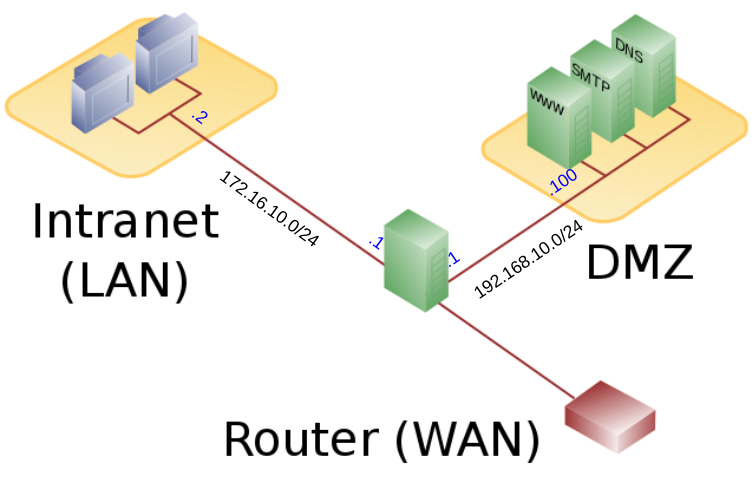
\includegraphics[scale=0.4]{img/esquema_red.png}
  \caption{Esquema de red}
  \label{fig:esquema de red}
\end{figure}

La configuración de red de cada máquina se muestra a continuación:
\begin{itemize}
  \item Maquina 1: \emph{Firewall}
  \begin{verbatim}
    # The primary network interface
    allow-hotplug ens3
    iface ens3 inet dhcp
    
    # The second network interace -> Server
    auto ens4
    iface ens4 inet static
            address 192.168.10.1
            netmask 255.255.255.0
    
    # The third network interface -> Client
    auto ens7
    iface ens7 inet static
            address 172.16.10.1
            netmask 255.255.255.0
  \end{verbatim}

  \item Maquina 2: \emph{Servidor}
  \begin{verbatim}
    # The primary network interface
    allow-hotplug ens3
    iface ens3 inet dhcp

    # The second network interface
    auto ens4
    iface ens4 inet static
            address 192.168.10.100
            netmask 255.255.255.0
            gateway 192.168.10.1
  \end{verbatim}

  \item Maquina 2: \emph{Cliente}
  \begin{verbatim}
    # The primary network interface
    allow-hotplug ens3
    iface ens3 inet dhcp

    # The second network interface
    auto ens4
    iface ens4 inet static
        address 172.16.10.2
        netmask 255.255.255.255
        gateway 172.16.10.1
  \end{verbatim}
\end{itemize}

% Nueva página 
\cleardoublepage

% Capitulo 2
\chapter{Configuracion de la red interna y un servidor en la DMZ}
Para este apartado se configura la red interna y se instala un servidor web en la DMZ. 
Primero debemos instalar en el cliente un navegor web, en este caso se instala \emph{links} 
con el comando \emph{sudo apt-get install links}. Luego, instalamos el servidor web \emph{nginx}
con el comando \emph{sudo apt-get install nginx}. 

Una vez instalado \emph{nginx} se procede a configurar el servidor web. Para ello, se accede al fichero \\
\emph{/etc/nginx/sites-available/default} y se modifica el fichero de la siguiente manera:

\begin{verbatim}
server {
  listen 192.168.10.100:80;
  server_name 10.6.129.251;
}
\end{verbatim}

Una vez modificado el fichero, se reinicia el servidor web con el comando \emph{sudo systemctl restart nginx}. Ya 
con el servidor web configurado, configuramos las reglas firewall para permitir la redirección de tráfico del puerto
80 al servidor web. Para ello, ejecutamos las siguientes reglas \emph{iptable} en el firewall:

\begin{verbatim}
iptables -t nat -A PREROUTING -i ens3 -p tcp --match multiport --dports 80,443 -j DNAT 
--to 192.168.10.100:80

iptables -t nat -A PREROUTING -i ens4 -d 10.6.129.251 -p tcp --match multiport 
--dports 80,443 -j DNAT --to 192.168.10.100:80
\end{verbatim}

Ya con el servidor web configurado y las reglas iptables configuradas, se procede a comprobar que el servidor web
funciona correctamente.


% Nueva página
\cleardoublepage

% Capitulo 3
\chapter{Configuración del Firewall con políticas por defecto DROP}
El script de configuración del firewall se muestra a continuación:

\begin{verbatim}
#!/bin/bash

# Reset all tables
iptables -P INPUT DROP
iptables -P FORWARD DROP
iptables -P OUTPUT ACCEPT
iptables -F
iptables -X
iptables -Z
iptables -t nat -F
iptables -t nat -X
iptables -t nat -Z

iptables -A FORWARD -i ens4 -p tcp --match multiport --dports 80,443 -j ACCEPT
iptables -A FORWARD -i ens7 -p tcp --match multiport --dports 80,443 -j ACCEPT

iptables -A FORWARD --match state --state ESTABLISHED,RELATED -j ACCEPT
iptables -A FORWARD -i ens3 -o ens7 -p tcp --match multiport --dports 80,443 -j ACCEPT

iptables -A FORWARD -p udp --dport 53 -j ACCEPT
iptables -A FORWARD -p udp --dport 53 -j ACCEPT

iptables -t nat -A POSTROUTING -o ens3 -j MASQUERADE
\end{verbatim}

En el punto de permitir tráfico web desde Internet al servidor web de la DMZ, aqui una captura de pantalla de la
página web de \emph{nginx} desde un navegador:

\begin{figure}[H]
  \centering
  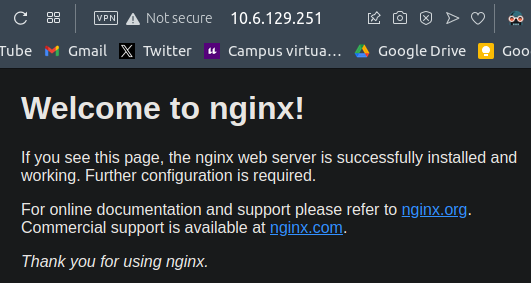
\includegraphics[scale=0.55]{img/nginx_navegador.png}
  \caption{Página web de nginx desde un navegador}
  \label{fig:página web de nginx desde un navegador}
\end{figure}

% Nueva página
\cleardoublepage

Luego, para el punto de permitir tráfico web desde red interna a al servidor web que está en la DMZ, una captura de pantalla
accediendo al servidor web con la IP privada, 192.168.10.100, desde el cliente:
q
\begin{figure}[H]
  \centering
  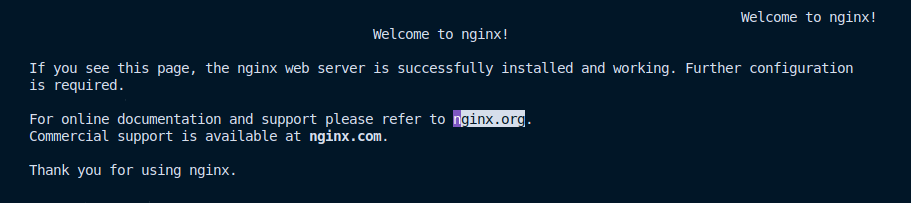
\includegraphics[scale=0.5]{img/nginx_cliente_privada.png}
  \caption{Página web de nginx desde el cliente con la IP privada}
  \label{fig:página web de nginx desde el cliente con la IP privada}
\end{figure}

\end{document}